\documentclass{article}
\usepackage[utf8]{inputenc}
\usepackage{graphicx}

\title{Introduzione all'Intelligenza Artificiale 2022}
\author{Ambra Manattini}
\date{February 2022}

\begin{document}

\maketitle

\section{Agenti Intelligenti}
Primo obiettivo: agenti per la risoluzione di problemi vista come ricerca in uno spazio di stati (\textbf{problem solving})

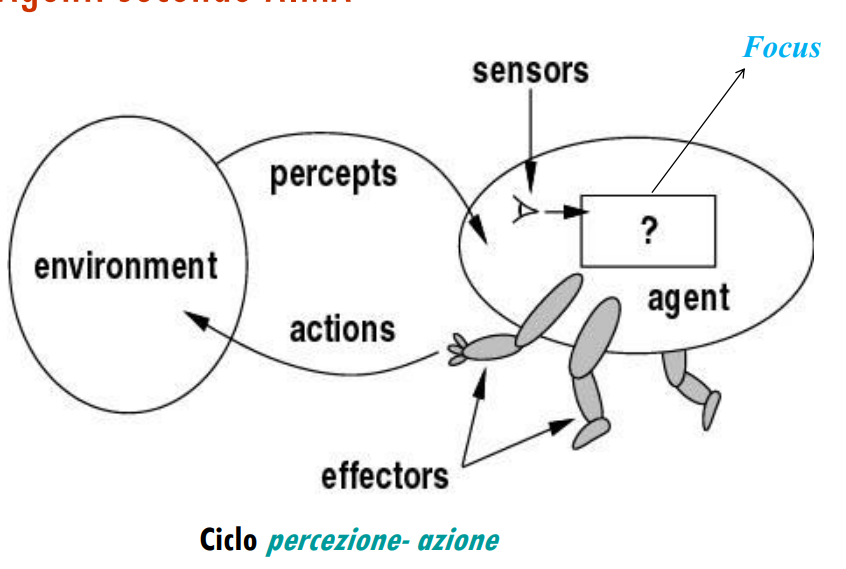
\includegraphics[width=\linewidth]{1.png}

L'agente esegue il ciclo percezione-azione. Il focus è il programma dell'agente

\subsection{Caratteristiche degli agenti}
\begin{enumerate}
    \item \textbf{Situati}: ricevono percezioni dall'ambiente e agiscono mediante \textit{azioni}
    \item \textbf{Abilità sociale}
    \item Credenze, obiettivi intenzioni
    \item Hanno un corpo fisico, fino a considerare i meccanismi delle emozioni
\end{enumerate}

La scelta dell'agente è una funzione della sequenza percettiva, definisce l'azione da compiere in base a ogni sequenza percettiva


\includegraphics[]{2.png}

\subsection{Agenti Razionali}
Un agente razionale interagisce col suo ambiente in maniera efficace, perché serve un criterio di valutazione oggettivo dell'effetto delle azione dell'agente (es costo minimo di un cammino alla soluzione)
\\


\textbf{Valutazione della prestazione}

Misura di prestazione
\begin{enumerate}
    \item Esterna (come vogliamo che il mondo evolva
    \item Scelta dal progettista a seconda del problema
    \item Possibilmente valutata su ambienti diversi
\end{enumerate}
La razionalità dipende da
\begin{enumerate}
    \item Misura di prestazione
    \item Conoscenza pregressa dell'ambiente
    \item Percezioni presenti e passate
    \item Capacità dell'agente
\end{enumerate}
Un agente razionale per ogni sequenza di percezioni compie l'azione che massimizza il valore atteso della misura delle prestazioni, considerando le sue percezioni passate e la sua conoscenza pregressa.
Raramente tutta la conoscenza dell'ambiente può essere fornita a priori, l'agente razionale deve essere in grado di modificare il suo comportamento con l'esperienza (\textit{si adatta})



\end{document}
